\section{Deducción de O(n) 1}
Deduzca formalmente $O(n)$, mostrando claramente su procedimiento,
para la siguente función:

\begin{lstlisting}[style=miEstilo, numbers=none]
int recursiva1(int n)
{
   if(n<=1)
      return 5;
   else
      return recursiva1(n/2) + recursiva1(n/2);
}
\end{lstlisting}

\[ T(recursiva1(n))=T(n)\]
$$$$
\begin{equation*}
  \label{eq:definicion-por-partes1}
  T(n) = \left\{
    \begin{array}{ll}
      \mathrm{si\ } n \le 1 \; :    &  T(comp_{if})+T(return)=2t\\
      &\\
      \mathrm{si\ } n > 1 \; : &  T(comp_{if})+T(return)+T(n/2)+T(n/2)\\
               & =\;t+t+2T(n/2)\\
               & =\;2t+2T(n/2)
    \end{array}
  \right.
\end{equation*}

Expandiendo parte recursiva:
\begin{eqnarray*}
  \label{eq:1}
  T(n)&=&\mathbf{2t}+2\,T(n/2)\\
  &=&2t+2[2t+2T(n/4)]=2t+4t+4T(n/4)=\mathbf{6t}+4\,T(n/4)\\
  &=&6t+4[2t+2T(n/8)]=6t+8t+8T(n/8)=\mathbf{14t}+8\,T(n/8)\\
  &=&14t+8[2t+2T(n/16)]=14t+16t+16T(n/16)=\mathbf{30t}+16\,T(n/16)\\
  &=&30t+16[2t+2T(n/32)]=30t+32t+32T(n/32)=\mathbf{62t}+32\,T(n/32)
\end{eqnarray*}

las partes en negrita de las expansiones puede escribirse tambien como
\begin{eqnarray*}
  2t&=&2t\\
  6t&=&2t+4t\\
  14t&=&2t+4t+8t\\
  30t&=&2t+4t+8t+16t\\
  62t&=&2t+4t+8t+16t+32t
\end{eqnarray*}

y para un k-ésimo término
$$t\,\sum_{x=1}^k2^x$$

dado que para cada número natural $n$, $2^0+2^1+2^2 \ldots +2^n=2^{n+1}-1$, la
enterior sumatoria queda

\begin{eqnarray*}
  t\,\sum_{x=1}^k2^x&=&t(2^0+2^1+2^2 + 2^3 \ldots +2^k \textcolor{green}{-1})\\
  &=&t(2^{k+1}-1 \textcolor{green}{-1})\\
  &=&t(2^{k+1}-2)\\
  &=&t(2^k2-2)\\
  &=&2t(2^k-1)
\end{eqnarray*}

el $\textcolor{green}{-1}$ restado a la ecuacion es para anular el $2^0$ de la secuencia
y así quede igual a la secuencia que es necesaria.

ahora para un k-ésimo término de la funcion $T(n)$ completa sería
\begin{equation}
  \label{eq:2}
  T(n)=2t(2^k-1)+2^k\,T(n/2^k)
\end{equation}

condicion de salida

\begin{eqnarray*}
  \label{eq:3}
  \frac{n}{2^k}&=&1\\
  n&=&2^k\\
  \log_{2}n&=&\log_{2}2^k\\
  k&=&\log_{2}n
\end{eqnarray*}

sustituyendo $k$ en \ref{eq:2} 

\begin{eqnarray*}
  T(n)&=&2t(2^{\log_{2}n}-1)+2^{\log_{2}n}\,T(n/2^{\log_{2}n})\\
  &=&2t(n-1)+n\,T(n/n)\\
  &=&2t(n-1)+n\,T(1)\\
  &=&2t(n-1)+n\,(2t) \;\;\;\;  \setminus \text{usando la parte no recursiva de T(n)}\\
  &=&2t(n-1+n)\\
  &=&2t(2n-1) \;\;\;\;  \setminus \text{por definición, tiempo minimo igual a 1 (t=1)}\\
  &=&4n-2
\end{eqnarray*}

deduciendo O(n)

\begin{eqnarray*}
  O[T(recursiva1(n))]&=&O[4n-2]\\
  &=&max(O(4n), O(-2))\\
  &=&O(4n)\\
  &=&n
\end{eqnarray*}
es lineal.

\section{Deducción de O(n) 2}
Deduzca formalmente $O(n)$, mostrando claramente su procedimiento,
para la siguiente función:
\begin{lstlisting}[style=miEstilo, numbers=none]
int recursiva2(int n){
  if(n<=1)
     return 5;
  else
     return recursiva2(n/3)
}
\end{lstlisting}

\[ T(recursiva2(n))=T(n)\]
$$$$
\begin{equation*}
  \label{eq:definicion-por-partes2}
  T(n) = \left\{
    \begin{array}{ll}
      \mathrm{si\ } n \le 1 \; :    &  T(comp_{if})+T(return)=2t\\
      \mathrm{si\ } n > 1 \; : &  T(comp_{if})+T(return)+T(llamadaRecursiva)=2t+T(n/3)
    \end{array}
  \right.
\end{equation*}

Expansión de parte recursiva:
\begin{eqnarray*}
  \label{eq:4}
  T(n)&=&2t+T(n/3)\\
      &=&2t+[2t+T((n/3)/3)]=2t+2t+T(n/9)=4t+T(n/9)\\
      &=&4t+[2t+T((n/9)/3)]=4t+2t+T(n/27)=6t+T(n/27)\\
      &=&6t+[2t+T((n/27)/3)]=6t+2t+T(n/81)=8t+T(n/81)
\end{eqnarray*}

para un k-esimo termino
\begin{equation}
  \label{eq:5}
  T(n)=2kt+T(n/3^k)
\end{equation}

condicion de salida
\begin{eqnarray*}
  \label{eq:6}
  \frac{n}{3^k}&=&1\\
  n&=&3^k\\
  \log_{3}(n)&=&\log_{3}(3^k)\\
  k&=&\log_{3}(n)
\end{eqnarray*}

sustituyendo k en (\ref{eq:5})

\begin{eqnarray*}
  T(n)&=&2\log_{3}(n)t+T(n/3^{\log_{3}(n)})\\
  &=&2\log_{3}(n)t+T(n/n)\\
  &=&2\log_{3}(n)t+T(1)\\
  &=&2\log_{3}(n)t+2t \;\;\;\;  \setminus \text{usando la parte no recursiva de T(n)}\\
  &=&2t(\log_{3}(n)+1)\\
  &=&2(\log_{3}(n)+1)\;\;\;\;  \setminus \text{por definición, tiempo minimo igual a 1 (t=1)}
\end{eqnarray*}

deduciendo O(n)

\begin{eqnarray*}
  O[T(recursiva2(n))]&=&O[T(n)]\\
  &=&O[2*(\log_{3}n+1)]\\
  &=&O[\log_{3}n+1]\\
  &=&max[O(\log_{3}n), O(1)]\\
  &=&O[\log_{3}n]\\
  &=&\log_{3}n
\end{eqnarray*}
tiene forma logaritmica


\section{Deducción de O(n) 3}
Deduzca formalmente $O(n)$, mostrando claramente su procedimiento,
para la siguiente función:
\begin{lstlisting}[style=miEstilo, numbers=none]
int iterativa(int n){
  int x=1; //s1
  while (x<=n){ //s2
    x*=3;
  }
  return x; //s3
}
\end{lstlisting}

\begin{eqnarray*}
  T[iterativa(n)] &=& T(n)\\
  T(n)&=&T(s1)+T(s2)+T(s3)\\
  T(n)&=&t+T(s2)+T(s3)\\
  T(n)&=&t+T(s2)+T(return)\\
  T(n)&=&t+T(s2)+t\\
  T(n)&=&2t+T(s2)\\
  T(n)&=&2t+T(while)\\
  T(n)&=&2t+v*[T(condicion)+T(cuerpoDelWhile)]\\
  T(n)&=&2t+v*(t+t)\\
  T(n)&=&2t+2t*v\\
  T(n)&=&2t(1+v)\\
\end{eqnarray*}

$v$=número de veces que se ejecuta el cuerpo y condición del while.

¿cuánto es $v$ en términos de $n$\footnote{$n$ representa el numero de
  datos que recibe el argoritmo}?

Podemos hacer un algoritmo equivalente
\begin{verbatim}
int iterativaEq(int n) {
    x=1 ;
    v=0 ;
    while (x <= n) {
        x *= 3 ;
        v = v + 1 ;
    }
    cout << "v=" << v ;
    return x;
}
\end{verbatim}
Valores de $v$ y $x$ respecto a $n$

\begin{tabular}{c|c|c|c}
  n & v & x $\leq$ n & iteraciones\\ \hline
  0 & 0 & 1 $\leq$ 0 & \\
  1 & 0 & 1 $\leq$ 1, 3 $\leq$ 1 & I\\
  2 & 1 & 1 $\leq$ 2, 3 $\leq$ 2 & I\\
  3 & 2 & 1 $\leq$ 3, 3 $\leq$ 3, 9 $\leq$ 3 & II\\
  4 & 2 & 1 $\leq$ 4, 3 $\leq$ 4, 9 $\leq$ 4 & II\\
  5 & 2 &   & II\\
  6 & 2 &   & II\\
  7 & 2 &   & II\\
  8 & 2 &   & II\\
  9 & 3 & 1$\leq$9, 3$\leq$9, 9$\leq$9, 27$\leq$9 & III\\
  10 & 3 & 1$\leq$10, 3$\leq$10, 9$\leq$10, 27$\leq$10 & III\\
  11 & 3 & 1$\leq$11, 3$\leq$11, 9$\leq$11, 27$\leq$11 & III\\
  \vdots & \vdots & \vdots & \vdots\\
  27 & 4 & 1$\leq$27, 3$\leq$27, 9$\leq$27, 27$\leq$27, 81$\leq$27&IV\\
\end{tabular}
\\[.5cm]
Podemos deducir que existe una relación entre $v$ y $n$ así:
$$n <  3^v$$

por tanto
\begin{eqnarray*}
  \log_3n &<&\log_33^v\\
  \log_3n&<&v
\end{eqnarray*}

retomando la función del tiempo anterior
\begin{eqnarray*}
  T(n)&=&2t(1+v)\\
  T(n)&=&2t(1+\log_3n)\\
  T(n)&=&2(1+\log_3n)\;\;\;\;  \setminus \text{por definición, tiempo minimo igual a 1 (t=1)}
\end{eqnarray*}

la función O(n) sería
\begin{eqnarray*}
  O[iterativa(n)] &=& O[T(n)]\\
                  &=& O[2(1+\log_3n)]\\
                  &=& O[1+\log_3n]\;\;\;\;  \setminus \text{regla de las constantes}\\
                  &=& max[O(1), O(\log_3n)]\\
                  &=&O(\log_3n)\\
                  &=& \log_3n
\end{eqnarray*}

tiene forma logaritmica.



\section{Mapeo de matriz triangular inversa}
\label{sec:matr-triang-inversa}

Una matriz triangular inversa se define como aquella matriz en la que
las posiciones $A[i,j]$ no existan cuando $j>n-i+1$, de modo que sólo
se utiliza la memoria necesaria para los elementos que sí se
usan. Deduzca formalmente la fórmula de mapeo lexicográfico
$LOC(A[i,j])$ para una matriz triangular inversa de pares límites $1
\ldots n$ (índice máximo $n$ e indice mínimo 1). Por ejemplo, para el
caso $n=3$.

\begin{equation*}
  \label{m-triangular-inversa}
    \begin{array}{|l|l|l|}
      \hline
      A[1,1]&A[1,2]&A[1,3]\\
      \hline
      A[2,1]&A[2,2]&\\
      \hline
      A[3,1]&&\\
      \hline
    \end{array}
\end{equation*}

Debe representarse en memoria así:

\begin{equation*}
  \begin{array}{|l|l|l|l|l|l|}
    \hline
    A[1,1]&A[1,2]&A[1,3]&A[2,1]&A[2,2]&A[3,1]\\
    \hline
  \end{array}
\end{equation*}

$$\mathbf{Loc(i, j)=\alpha+AvanceFilas+AvanceColumnas}$$

A simple vista se puede deducir que el avance en columnas es
\textbf{j-1}.

Dado que si seleccionamos la posición $A[1,3]$ el avance en filas es 0
y la posición del arreglo correspondiente al mapeo es la posición
$2$. $(3-1=2)$.

Para deducir el avance en filas debemos observar el patrón, tomando
como $N$ el tamaño de la primera fila:

\begin{equation*}
  \begin{array}{|l|l|}
    \hline
    i&\text{Avance}\\
    \hline
    1&0\\
    \hline
    2&N\\
    \hline
    3&N+N-1\\
    \hline
    4&N+N-1+N-2\\
    \hline
    5&N+N-2+N-2+N-3\\
    \hline
    k&N+N-2+N-2+N-3 \ldots N-(k-2) \\
    \hline
  \end{array}
\end{equation*}

Lo cual se puede representar con la siguiente sumatoria:
$$\sum_{k=0}^{i-2} N-k$$

Por lo tanto la fórmula de mapeo lexicográfico para una matriz
triangular inversa es:
$$Loc(i,j)=\alpha+\sum_{k=0}^{i-2}(N-k)+(j-1)$$

\section{Mapeo de matriz triangular}
\label{sec:mapeo-de-matriz}

Una matriz triangular se define como aquella matriz en la que las
posiciones $A[i,j]$ no existan cuando $j>i$, de modo que sólo se
utiliza la memoria necesaria para los elementos que sí se
usan. Deduzca la fórmula de mapeo lexicográfico $LOC(A[i,j])$ para una
matriz triangulares de índice máximo $n$ e índice mínimo $1$. Por
ejemplo, para el caso $n=3$:

\begin{equation*}
  \label{m-triangular-inversa}
    \begin{array}{|l|l|l|}
      \hline
      A[1,1]& &\\
      \hline
      A[2,1]&A[2,2]&\\
      \hline
      A[3,1]&A[3,2]&A[3,3]\\
      \hline
    \end{array}
\end{equation*}

Debe representarse en memoria así:

\begin{equation*}
  \begin{array}{|l|l|l|l|l|l|}
    \hline
    A[1,1]&A[2,1]&A[2,2]&A[3,1]&A[3,2]&A[3,3]\\
    \hline
  \end{array}
\end{equation*}


\begin{eqnarray*}
  \mathbf{Loc(A[i,j])}&=& \mathbf{ a + NumPosicionesAntesDeFila(i)+AvanzarAColumna(j)}\\
  &=&\alpha+NumPosicionesAntesDeFila(i)+(j-1)\\
  &=&\alpha+\sum_{x=1}^{i-1}x+(j-1)
\end{eqnarray*}

dado que para un entero $n$ lo siguiente es cierto:
$1+2+3+4+\ldots+n=n(n+1)/2$. La funcion de mapeo queda

\begin{eqnarray*}
  \mathbf{Loc(A[i,j])}&=&\alpha+\sum_{x=1}^{i-1}x+(j-1)\\
  &=&\alpha+\frac{(i-1)[(i-1)+1]}{2}+(j-1)\\
  &=&\alpha+\frac{(i-1)[i-1+1]}{2}+(j-1)\\
  &=&\alpha+\frac{i(i-1)}{2}+j-1
\end{eqnarray*}



\section{Multiplicación de una matriz lexicográfica.}
\label{sec:mult-de-una}
Dado el siguiente código:
\begin{lstlisting}[style=miEstilo, numbers=none]
using namespace std;

class Matriz{
public:
    Matriz(int n[], int m[]);//* constructor con los pares límites
    virtual ~Matriz();//* destructor

    /** se ponen y obtienen valores */
    int &operator[](int i[]);

    //* crea una nueva matriz, que la multiplicacion de esta matriz por el m
    Matriz *operator* (Matriz m);
};

int main(){
    cout << "Multiplicacion" << endl;

    /* se define la matriz m1: 10..12 * 1..4 */
    Matriz m1({10,1},{12,4});

    /* se define la matriz m2: 11..14 * 1..5*/
    Matriz m2({11,1}, {14,5});

    /* se inicializan algunas posiciones */
    m1[10,2]=1;
    m1[12,4]=1;
    m2[12,3]=1;
    m2[14,4]=1;

    /* se obtiene la matriz resultado de la multiplicacion
     * m3=10..12 * 1..5
     */

    Matriz *m3=m1*m2;

    /* se imprime la matriz resultante */
    for(int i=10;i<=12;i++){
        for(int j=1;j<=5;j++){
            cout << "["<<i<<","<<j<<"]="<<m3[{i,j}]; << " -- ";
        }
        cout << endl;
    }
    delete m3;
    return 0;
}
\end{lstlisting}

\begin{itemize}
\item[a)] Desarrolle los métodos necesarios en la clase Matriz para la
  implementación de la multiplicación (\textbf{operator*}) para una
  matriz lexicográfica.
\item [b)] Deduzca O(n) para el método \textbf{operator*}.
\end{itemize}

\section{Matriz esparcida}

Una aplicación de hoja electrónica, maneja la matriz de celdas como
una matriz esparcida, con dos vectores de apuntadores a elementos de
lista ortogonal. Uno de los vectores se indiza de la A a la Z y sirve
para puntos de entrada a las columnas, el otro se indiza de 1 a 256 y
sirve para puntos de entrada para las filas. Escriba una rutina
\textbf{Move(int F1, char C1, int F2, char C2, int FD, char CD)} que
mueva el rango especificado por las esquinas \textbf{(F1, C1)} y
\textbf{(F2, C2)} al rango que comienza en \textbf{(FD, CD)} solamente
moviendo las celdas de lugar, es decir, sin crear nuevos nodos.

\begin{center}
  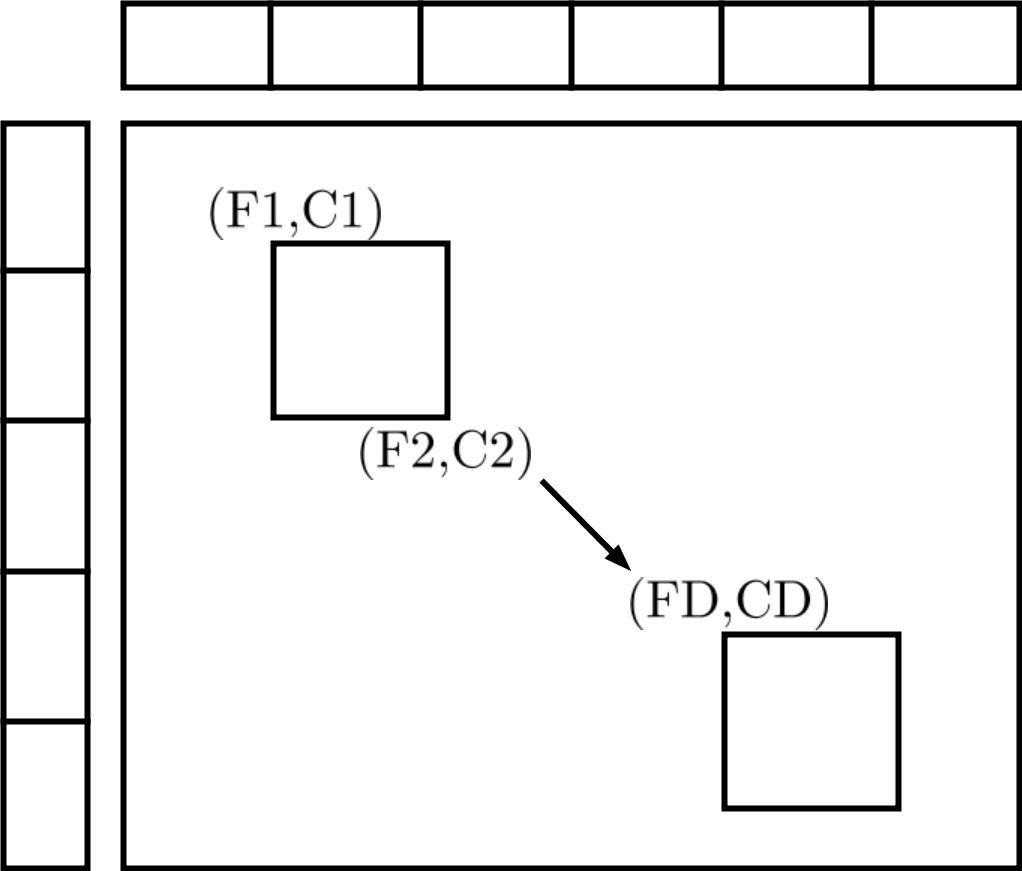
\includegraphics[scale=.2]{hojaCalculo.jpg}
\end{center}

\section{Árbol de expresiones}
\label{sec:arbol-de-expresiones}

Dada una clase ArbolExp, que representa un árbol de expresiones,
escriba un método \textbf{valor()} que de como resultado el valor de
la expresión representada. Puede suponer que sólo existen los
operadores de suma, resta, muliplicación y división. También se supone
que todos los operandos son constantes, es decir no hay variables. No
debe utilizar ninguna estructura de datos adicional. Suponga que sólo
existen las siguientes variables en cada clase:
\begin{lstlisting}[style=miEstilo, numbers=none]
class ArbolExp{
public:
   ...
   int valor();
   ...
private:
   NodoExp *raiz;
   ...
};

class NodoExp{
   ...
   void *valor;//constante u operador
   NodoExp *izq;
   NodoExp *der;
   ...
};
\end{lstlisting}

La solución es la siguiente:
\begin{lstlisting}[style=miEstilo, numbers=none]
  int ArbolExp::valor(){
    return valor(raiz);
  }

  int ArbolExp::valor(NodoExp* n){
    char * s;

    if(n==NULL)
      return -1;

    s=(char *) n->valor;//se asume que valor apunta a una cadena

    if(strcmp(s,"*")==0)
      return valor(n->izq)*valor(n->der);
    else if(strcmp(s,"/")==0)
      return valor(n->izq)/valor(n->der);
    else if(strcomp(s,"+")==0)
      return valor(n->izq)+valor(n->der);
    else if(strcmp(s,"-")==0)
	return valor(n->izq)-valor(n->der);
    else
      return atoi(s);
  }
\end{lstlisting}


\section{Tabla de Hash}
\label{sec:tabla-de-hash}

Explique los cuatro elementos generales de una tabla de dispersión.

\begin{description}
\item[Tabla: ] En esta se guarda los elementos del universo.
\item[Función Hash: ] También conocida como funcion de dispersión y da
  la posición en la tabla para una llave pasada como parámetro.
\item[Colisiones: ] Ocurre cuando dos llaves distintas dan posiciones
  de tabla coincidentes. Se debe adoptar alguna política de resolución
  de colisiones, como encadenamiento simple por ejemplo, para
  solucionarlo.
\item[Universo: ] Son elementos que posiblemente se añadirán en la
  tabla y no necesariamente ocupan espacio de memoria.
\end{description}


\section{Direccionamiento abierto de doble dispersión}

En una tabla de dispersión de tamaño $M=13$, con $h(llv)=llv \;mod\; M$,
$S(llv,i)=(llv \;mod\; 7\; + \;1)*i$, y utilizando direccionamiento abierto de
doble dispersión, realice la inserción de las siguientes llaves:
15,26, 29,2,18,28.

\begin{itemize}
\item Tamaño M=13
\item Función de dispersión $h(llv)=llv\; mod \;M$
\item Función de doble dispersión $S(llv,i)=(llv \;mod\; 7+1)$
\end{itemize}


\begin{figure}[H]
  \centering
  \begin{tabular}{|c|c|c|c|c|}
    \hline 
    LLave & $h(llv)$ & $h(llv)+S(llv,1)$ & $h(llv)+S(llv,2)$ &Posición final\\
    \hline
    16    & 15 mod 13=2 & No hay colisión       & No hay colisión &  2\\
    26    & 26 mod 13=0 & No hay colisión       & No hay colisión &  0\\
    29    & 19 mod 13=3 & No hay colisión       & No hay colisión &  3\\
    2     &  2 mod 13=2 & 2+(2 mod 7 + 1)*1=5   & No hay colisión &  5\\
    18    & 18 mod 13=5 & 5+(18 mod 7 + 1)*1=10 & No hay colisión &  10\\
    28    & 28 mod 13=2 & 2+(28 mod 7 + 1)*1=3  & 2+(28 mod 7 + 1)*2=4& 4\\
    \hline
  \end{tabular}
  \caption{Insertando valores}
\end{figure}


\begin{figure}[H]
  \centering
  \begin{tabular}{|c|}
    \hline
    26\\
    \hline
    \\
    \hline
    15\\
    \hline
    29\\
    \hline
    28\\
    \hline
    2\\
    \hline
    \\
    \hline
    \\
    \hline
    \\
    \hline
    \\
    \hline
    28\\
    \hline
    \\
    \hline
    \\
    \hline
  \end{tabular}
  \caption{Tabla resultante}
\end{figure}

\section{Búsqueda de texto}

Describa paso a paso, las distintas comparaciones o corrimientos, que
se realizaría al buscar el patrón ''\textbf{ABDCDE}'' en el texto
''\textbf{ABXDEEEBDEAABDE}'' usando la búsqueda de Booyer-Moore.

\section{Criptografía}

Con una técnica de criptografía pública, definimos $E(P_{pbl},T)$ como
el encriptado del texto $T$ con llave pública $P_{pbl}$ de la persona
$P$ y $E(P_{prv},T)$ como el encriptado del texto $T$ con la llave
privada $P_{prv}$ de la persona P. Tambíen definimos $D(P_{pbl},C)$
como el desencriptado del criptograma $C$ con la llave pública
$P_{pbl}$ de la persona $P$ y $D(P_{prv},C)$ como el desencriptado del
criptograma $C$ con la llave privada $P_{prv}$ de la persona $P$. Si
una persona $X$ desea enviar un mensaje a un sujeto $Y$, de modo que
$X$ esté seguro que sólo $Y$ podrá leer el mensaje y $Y$ esté seguro
que sólo $X$ pudo haber enviado el mensaje. Indique cómo $X$ deberá
encriptar el mensaje y cómo $Y$ deberá desencriptarlo pra lograr este
objetivo.

La \textbf{solución} es la siguiente: la persona $X$ encripta así:
\begin{eqnarray*}
  C_1&=& E(X_{prv},T)\\
  C_2&=&E(Y_{pbl},C_1)
\end{eqnarray*}

la persona $Y$ desencripta así:
\begin{eqnarray*}
  C_1&=& D(Y_{prv},C_2)\\
  T&=&D(X_{pbl},C_1)
\end{eqnarray*}

%%% Local Variables:
%%% mode: latex
%%% TeX-master: "tedd"
%%% End:
